%%-----------------------------------------------------------------------%%
%%--- Trees and Forests -------------------------------------------------%%

\chapter{Trees and Forests}
\label{chap:trees_forests}

In section~\ref{subsec:introduction:walks_trails_paths}, we briefly
touched upon trees and provided examples of how trees could be used to
model hierarchical structures. This chapter provides an in-depth study
of trees, their properties, and various applications.

{\color{red}{
\begin{itemize}
\item Discuss heaps and how these relate to realizing efficient
  implementations of Dijkstra's
  Algorithm~\ref{alg:graph_algorithms:dijkstra_general}.
\end{itemize}
}
}


%%-----------------------------------------------------------------------%%
%%--- Definitions and examples ------------------------------------------%%

\section{Definitions and examples}

Recall that a path in a graph $G = (V, E)$ whose start and end vertices
are the same is called a cycle. We say $G$ is
\emph{acyclic}\index{acyclic}, or a \emph{forest}\index{forest}, if it
has no cycles. In a forest, a vertex of degree one is called an
\emph{endpoint}\index{endpoint} or a \emph{leaf}\index{leaf}. A
connected forest is a \emph{tree}\index{tree}.

A \emph{rooted tree}\index{tree!rooted} is a tree with a specified
\emph{root}\index{root} vertex $v_0$. (However, if $G$ is a rooted
tree with root vertex $v_0$ having degree one then, by convention, we
do not call $v_0$ an endpoint or a leaf.) The Unix\index{Unix}, in
particular Linux\index{Linux}, filesystem\index{filesystem} hierarchy
can be viewed as a tree~(see
Figure~\ref{fig:trees_forests:filesystem_hierarchy}). As shown in
Figure~\ref{fig:trees_forests:filesystem_hierarchy}, the root vertex
is designated with the forward slash, which is also referred to as the
root directory\index{root directory}.

\begin{figure}[!htbp]
\centering
\begin{tikzpicture}
\node {\texttt{/}} [edge from parent fork down]
  child {node {\texttt{bin}}}
  child {node {\texttt{etc}}}
  child {node {\texttt{home}}
    child {node {\texttt{anne}}}
    child {node {\texttt{sam}}}
    child {node {$\dots$}}
  }
  child {node {\texttt{lib}}}
  child {node {\texttt{opt}}}
  child {node {\texttt{proc}}}
  child {node {\texttt{tmp}}}
  child {node {\texttt{usr}}
    child {node {\texttt{bin}}
      child {node {\texttt{acyclic}}}
      child {node {\texttt{diff}}}
      child {node {\texttt{dot}}}
      child {node {\texttt{gc}}}
      child {node {\texttt{neato}}}
      child {node {$\dots$}}
    }
    child {node {\texttt{include}}}
    child {node {\texttt{local}}}
    child {node {\texttt{share}}}
    child {node {\texttt{src}}}
    child {node {$\dots$}}
  }
  child {node {$\dots$}};
\end{tikzpicture}
\caption{The Linux filesystem hierarchy.}
\label{fig:trees_forests:filesystem_hierarchy}
\end{figure}

A \emph{directed tree}\index{tree!directed} is a digraph which would
be a tree if the directions on the edges were ignored. A rooted tree
can be regarded as a directed tree since we can imagine an edge
$E = uv$ for $u,v \in V$ being directed from $u$ to $v$ if and only
if $v$ is further away from $v_0$ than $u$ is. If $e = uv$ is an edge
in a rooted tree, then we call $v$ a \emph{child}\index{child} vertex
with \emph{parent}\index{parent} $u$. Directed trees are pervasive in
theoretical computer science, as they are useful structures for
describing algorithms and relationships between objects in certain
data sets.

An \emph{ordered tree}\index{tree!ordered} is a rooted tree for which
an ordering is specified for the children of each vertex. An
$n$-\emph{ary tree}\index{tree!$n$-ary} is a rooted tree for which
each vertex that is not a leaf has at most $n$ children. The case
$n = 2$ are called \emph{binary trees}\index{tree!binary}. A
\emph{spanning tree}\index{spanning tree} $T$ of a connected,
undirected graph $G$ is a subgraph containing all vertices of $G$
which is a tree.

\begin{example}
\label{example:span-tree}
{\rm
Consider the $4 \times 4$ grid graph with $16$ vertices and
$24$ edges. Two examples of a spanning tree are given in
Figure~\ref{fig:trees_forests:grid_graph_spanning_trees} by using
thicker line width for its edges.}
\hfill $\square$
\end{example}

\begin{figure}[!htbp]
\centering
\subfigure[]{
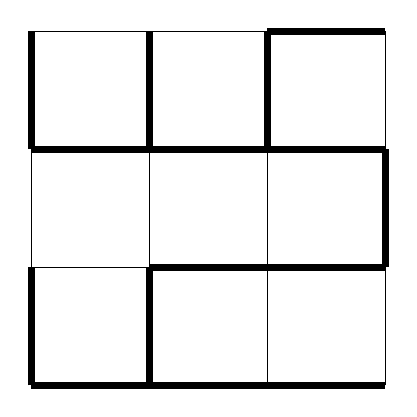
\begin{tikzpicture}
[linedecorate/.style={line width=2.5pt}]
%% set up the grid
\foreach \xstart/\xend/\y in {0/4.5/0, 0/4.5/1.5, 0/4.5/3, 0/4.5/4.5} {
  \draw (\xstart,\y) -- (\xend,\y);
  \draw (\y,\xstart) -- (\y,\xend);
}
%% draw the spanning tree
\foreach \xstart/\ystart/\xend/\yend in {0/0/0/1.5, 0/0/4.5/0,
  1.5/0/1.5/1.5, 1.5/1.5/4.5/1.5, 4.5/1.5/4.5/3, 0/3/4.5/3, 0/3/0/4.5,
  1.5/3/1.5/4.5, 3/3/3/4.5, 3/4.5/4.5/4.5} {
  \draw[linedecorate] (\xstart,\ystart) -- (\xend,\yend);
}
\end{tikzpicture}
}
%%
%%
\qquad
\subfigure[]{
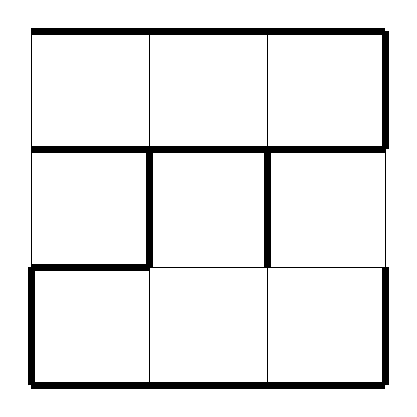
\begin{tikzpicture}
[linedecorate/.style={line width=2.5pt}]
\foreach \xstart/\xend/\y in {0/4.5/0, 0/4.5/1.5, 0/4.5/3, 0/4.5/4.5} {
  \draw (\xstart,\y) -- (\xend,\y);
  \draw (\y,\xstart) -- (\y,\xend);
}
%% draw the spanning tree
\foreach \xstart/\ystart/\xend/\yend in {0/0/0/1.5, 0/0/4.5/0,
  4.5/0/4.5/1.5, 0/1.5/1.5/1.5, 1.5/1.5/1.5/3, 3/1.5/3/3, 0/3/4.5/3,
  4.5/3/4.5/4.5, 0/4.5/4.5/4.5} {
  \draw[linedecorate] (\xstart,\ystart) -- (\xend,\yend);
}
\end{tikzpicture}
}
\caption{Spanning trees for the $4 \times 4$ grid graph.}
\label{fig:trees_forests:grid_graph_spanning_trees}
\end{figure}

The following game is a variant of the Shannon switching game, due to
Edmunds and Lehman\index{edge-tagging game}. We follow the description
in Oxley's survey ({\it What is a matroid?'}
{\color{red}{add reference later}}). Recall that a minimal edge cut of
a graph is also called a bond\index{bond} of the graph. The following
two-person game is played on a connected graph $G = (V,E)$. Two
players Alice and Bob alternately tag elements of $E$. Alice's goal is
to tag the edges of a spanning tree, while Bob's goal is to tag the
edges of a bond. If we think of this game in terms of a communication
network, then Bob's goal is to separate the network into pieces that
are no longer connected to each other, while Alice is aiming to
reinforce edges of the network to prevent their destruction. Each move
for Bob consists of destroying one edge, while each move for Alice
involves securing an edge against destruction.

\begin{theorem}
The following statements are equivalent for a connected graph $G$.
%
\begin{enumerate}
\item Bob plays first and Alice can win against all possible
  strategies of Bob.

\item The graph $G$ has 2 edge-disjoint spanning trees.

\item For all partitions $P$ of the vertex set $V$ of $G$, the number
  of edges of $G$ that join vertices in different classes of the
  partition is at least $2(|P| - 1)$.
\end{enumerate}
\end{theorem}

%%-----------------------------------------------------------------------%%
%%--- Properties of trees -----------------------------------------------%%

\section{Properties of trees}

%\begin{itemize}
%\item trees and acyclic graphs; leaves
%
%\item forests
%\end{itemize}

The following theorem gives several basic
characterizations of trees.

\begin{theorem}
If $T = (V, E)$ is a graph with $n$ vertices, then the following
statements are equivalent:
\begin{enumerate}
\item $T$ is a tree.

\item $T$ contains no cycles and has $n - 1$ edges.

\item $T$ is connected and has $n - 1$ edges.

\item Every edge of $T$ is a cut set.

\item For any $u,v \in V$, there is exactly one $u$-$v$ path.

\item For any new edge $e$, the join $T + e$ has exactly one cycle.
\end{enumerate}
\end{theorem}

Let $G=(V_1,E_2)$ be a graph and $T=(V_2,E_2)$ a subgraph of $G$ which is a tree.
As in (6) we see adding just one edge in $E_1-E_2$ to $T$ will create a
unique cycle in $G$. Such a cycle is called a {\it fundamental cycle}
of $G$. (The set of such fundamental cycles of $G$ depends on $T$.)
\index{fundamental cycle}
\index{tree}

\begin{proof}[Solution]
\noindent
(1) $\implies$ (2):
This basically follows by induction on the number of vertices.

By definition, a tree has no cycles. Make the following
induction hypothesis: for any tree $T=(V,E)$, $|E|=|V|-1$.
This holds in the base case where $|V|=1$ since in that case,
there can be no edges. Assume it is true for all trees with
$|V|=k$, for some $k>1$. Let $T=(V,E)$ be a tree having
$k+1$ vertices. Remove an edge (but not the vertices
it is incident to). This
disconnects
$T$ into $T_1=(V_1, E_1)$ union $T_2 = (V_2, E_2)$,
where $|E|=|E_1|+|E_2|+1$ and $|V|=|V_1|+|V_2|$
(and possibly one of the $E_i$ is empty),
each of which is a tree satisfying the conditions of the induction
hypothesis. Therefore,

\[
|E|=|E_1|+|E_2|+1 = |V_1| - 1 + |V_2| - 1 + 1 =|V|-1.
\]

\noindent
(2) $\implies$ (3):
If $T=(V,E)$ has $k$ connected components then it is a disjoint
union of trees $T_i=(V_i,E_i)$, $i=1,2,\dots, k$,
for some $k$. Each of these satisfy, by (2),

\[
|E_i|=|V_i|-1,
\]
so

\[
|E|=\sum_{i=1}^k |E_i|
=\sum_{i=1}^k |V_i| -k
=|V|-k.
\]
This contradicts (2) unless $k=1$.
Therefore, $T$ is connected.

\noindent
(3) $\implies$ (4):
If removing an edge $e\in E$ leaves $T=(V,E)$ connected then
$T'=(V,E')$ is a tree, where $E'=E-e$.
However, this means that $|E'|=|E|-1=|V|-1-1=|V|-2$,
which contradicts (3). Therefore $e$ is a cut set.

\noindent
(4) $\implies$ (5):
Let

\[
P = (v_0=u\to v_1 \to v_2 \to \dots \to v_k = v)
\]
and
\[
P' = (v'_0=u\to v'_1 \to v'_2 \to \dots \to v'_\ell = v)
\]
be two paths from $u$ to $v$.

\noindent
(5) $\implies$ (6):
Let $e=(u,v)$ be a new edge connecting $u,v\in V$.
Suppose that

\[
P = (v_0=w\to v_1 \to v_2 \to \dots \to v_k = w)
\]
and
\[
P' = (v'_0=w\to v'_1 \to v'_2 \to \dots \to v'_\ell = w)
\]
are two cycles in $T\cup (\{u,v\},\{e\})$.

If either $P$ or $P'$ does not contain $e$,
say $P$ does not contain $e$, then $P$ is a
cycle in $T$. Let $u = v_0$ and let $v=v_1$.
The edge $v_0=w\to v_1$ is a $u$-$v$ path
and the sequence $v=v_1 \to v_2 \to \dots \to v_k=w=u$
taken in reverse order is another $u$-$v$ path.
This is a contradiction to (5).

We may suppose now that $P$ and $P'$ both contain $e$.
Therefore, $P$ contains a subpath $P_0=P-e$ (which is not
closed), that is the same as $P$ except it lacks the edge
from $u$ to $v$. Likewise, $P'$ contains a subpath $P'_0=P'-e$ (which is not
closed), that is the same as $P'$ except it lacks the edge
from $u$ to $v$. By (5), these $u$-$v$ paths
$p_0$ and $P_0'$ must be the same. This forces
$P$ and $P'$ to be the same, which proves (6).


\noindent
(6) $\implies$ (1):
Condition (6) implies that $T$ is acyclic. (Otherwise, it is trivial
to make two cycles by adding an extra edge.) We must show $T$ is connected.
Suppose $T$ is disconnected. Let $u$ be a vertex in one component,
$T_1$ say,
of $T$ and $v$ a vertex in another component, $T_2$ say, of $T$.
Adding the edge $e=(u,v)$ does not create a cycle (if it did
then $T_1$ and $T_2$ would not be disjoint), which contradicts (6).
\end{proof}

\begin{exercise}
Let $G=(V_1,E_2)$ be a graph and $T=(V_2,E_2)$ a spanning tree of $G$.
Show there is a one-to-one correspondence between fundamental cycles in $G$ and
edges not in $T$.
\end{exercise}

\begin{exercise}
Let $G=(V, E)$ be the $3\times 3$ grid graph and $T_1=(V_1,E_1)$,
$T_2=(V_2,E_2)$ be spanning trees of $G$ in Example \ref{example:span-tree}.
Find a fundamental cycle in $G$ for $T_1$ which is not a
fundamental cycle in $G$ for $T_2$.
\end{exercise}

\begin{exercise}
Usually there exist many spanning trees of a graph.
Can you classify those graphs for which there is only one spanning tree?
In other words, find necessary and sufficient conditions for a
graph $G$ such that if $T$ is a spanning tree then $T$ is unique.
\end{exercise}


%%-----------------------------------------------------------------------%%
%%--- Minimum spanning trees --------------------------------------------%%

\section{Minimum spanning trees}

Suppose you want to design an electronic circuit
connecting several components. If these components represent the
vertices of the graph and a wire connecting two components
represents an edge of the graph then, for economical reasons, you will want to
connect these together using the least amount of wire.
This amounts to finding a minimum spanning tree in the
complete graph on these vertices.

\begin{itemize}
\item spanning trees

We can characterize a spanning tree in several ways. Each of these
conditions lead to an algorithm for constructing them.

One condition is that spanning tree of a connected graph $G$ can also
be defined as a maximal set of edges of $G$ that contains no cycle.
Another condition is that it is a minimal set of edges that connect
all vertices.

Exploiting the former criteria gives rise to Kruskal's algorithm.
Exploiting the latter criteria gives rise to Prim's algorithm.
Both of these argorithms are discussed in more detail below.

\item minimum-cost spanning trees

A {\it minimum spanning tree} (MST) is a spanning
tree of an edge weighted graph having lowest total weight
among all possible spanning trees.
\index{tree!minimum spanning}
\index{MST}

\item Kruskal's algorithm~\cite{Kruskal1956}; see also section~23.2 of
  Cormen~et~al.~\cite{CormenEtAl2001}.

Kruskal's algorithm is a greedy algorithm to compute a MST.
It was discovered by J. Kruskal in the 1950's.

Kruskal's algorithm can be shown to run in $O(|E| \log |E|)$ time.


\item Prim's algorithm~\cite{Prim1957}; see also section~23.2 of
  Cormen~et~al.~\cite{CormenEtAl2001}.

Prim's algorithm is a greedy algorithm to compute a MST. In can be
implemented in time $O(|E| + |V| \log |V|)$, which is
$O(n^2)$ for a dense graph having $n$ vertices.

The algorithm was developed in the 1930's by Czech mathematician V.
Jarn\'ik and later independently by both the computer scientists R. Prim
and E. Dijkstra in the 1950's.

\item Bor\r{u}vka's algorithm~\cite{Boruvka1926a,Boruvka1926b}

Bor\r{u}vka's algorithm is an algorithm for finding a minimum spanning
tree in a graph
for which all edge weights are distinct.
It was first published in 1926 by Otakar Bor\o uvka but then
rediscovered by many others.

Bor\r{u}vka's algorithm can be shown to run in time
$O(|E|\log |V|)$.


\end{itemize}

\subsection{Kruskal's algorithm}

Kruskal's algorithm starts with an edge-weighted digraph $G=(V,E)$
as input. Let $w:E\to {\mathbb{R}}$ denote the weight function.
The first stage is to create a ``skeleton'' of the
tree $T$ which is initially set to be a graph with no
edges: $T=(V,\emptyset)$. The next stage is to
sort the edges of $G$ by weight. In other words, we
label the edges of $G$ as

\[
E = \{e_1,e_2,\dots ,e_m\},
\]
where $w(e_1) \leq w(e_2) \leq \dots \leq w(e_m)$.
Next, start a for loop over $e\in E$. You add
$e$ to $T$ as an edge provided it does not create
a cycle. The only way adding $e=(u,v)$ to $T$ would
create a cycle would be if both $u$ and $v$ were
endpoints of an edge already in $T$. As long as this
cycle condition fails, you add $e$ to $T$ and otherwise,
go to the next element of $E$ in the for loop.
At the end of the for loop, the edges of $T$ have
been completely found and the algorithm stops.

\begin{center}
\vskip .15in

\begin{Verbatim}[fontsize=\scriptsize,fontfamily=courier,fontshape=tt,frame=single,label=\sage]

def kruskal(G):
    """
    Implements Kruskal's algorithm to compute a MST of a graph.

    INPUT:
        G - a connected edge-weighted graph or digraph
               whose vertices are assumed to be 0, 1, ...., n-1.
    OUTPUT:
        T - a minimum weight spanning tree.

    If G is not explicitly edge-weighted then the algorithm
    assumes all edge weights are 1. The tree T returned is
    a weighted graph, even if G is not.

    EXAMPLES:
        sage: A = matrix([[0,1,2,3],[0,0,2,1],[0,0,0,3],[0,0,0,0]])
        sage: G = DiGraph(A, format = "adjacency_matrix", weighted = True)
        sage: TE = kruskal(G); TE.edges()
        [(0, 1, 1), (0, 2, 2), (1, 3, 1)]
        sage: G.edges()
        [(0, 1, 1), (0, 2, 2), (0, 3, 3), (1, 2, 2), (1, 3, 1), (2, 3, 3)]
        sage: G = graphs.PetersenGraph()
        sage: TE = kruskal(G); TE.edges()
        [(0, 1, 1), (0, 4, 1), (0, 5, 1), (1, 2, 1), (1, 6, 1), (2, 3, 1),
         (2, 7, 1), (3, 8, 1), (4, 9, 1)]

    TODO:
        Add ''verbose'' option to make steps more transparent.
       (Useful for teachers and students.)
    """
    T_vertices = G.vertices() # a list of the form range(n)
    T_edges = []
    E = G.edges() # a list of triples
    # start ugly hack
    Er = [list(x) for x in E]
    E0 = []
    for x in Er:
        x.reverse()
        E0.append(x)
    E0.sort()
    E = []
    for x in E0:
        x.reverse()
        E.append(tuple(x))
    # end ugly hack to get E is sorted by weight
    for x in E:  # find edges of T
        TV = flatten(T_edges)
        u = x[0]
        v = x[1]
        if not(u in TV and v in TV):
            T_edges.append([u,v])
    # find adj mat of T
    if G.weighted():
        AG = G.weighted_adjacency_matrix()
    else:
        AG = G.adjacency_matrix()
    GV = G.vertices()
    n = len(GV)
    AT = []
    for i in GV:
        rw = [0]*n
        for j in GV:
            if [i,j] in T_edges:
                rw[j] = AG[i][j]
        AT.append(rw)
    AT = matrix(AT)
    return Graph(AT, format = "adjacency_matrix", weighted = True)

\end{Verbatim}

\end{center}
\index{Kruskal's algorithm}

Here are some examples.

We start with the grid graph. This is implemented in Sage
in a way that the vertices are given by the coordinates of the
grid the graph lies on, as opposed to $0,1,\dots,n-1$.
Since the above implementation assumes that the
vertices are $V=\{0,1,\dots,n-1\}$, we first redefine
the graph suitable and run the Kruskal algorithm on that.

\begin{center}
\fontsize{9pt}{9pt}
\selectfont
\tt
\begin{lstlisting}
sage: G = graphs.GridGraph([4,4])
sage: A = G.adjacency_matrix()
sage: G = Graph(A, format = "adjacency_matrix", weighted = True)
sage: T = kruskal(G); T.edges()
[(0, 1, 1), (0, 4, 1), (1, 2, 1), (1, 5, 1), (2, 3, 1), (2, 6, 1), (3,7, 1),
 (4, 8, 1), (5, 9, 1), (6, 10, 1), (7, 11, 1), (8, 12, 1), (9, 13, 1),
 (10, 14, 1), (11, 15, 1)]
\end{lstlisting}
\end{center}
%
The plot of this graph is given in
Figure~\ref{fig:trees-forests:Kruskal_example}.


\begin{figure}[h!]
\begin{center}
\unitlength=0.920000pt
\begin{picture}(210.00,192.00)(0.00,0.00)
%\put(-3.00,-3.00){$\bullet$} % vertices look funny
%\put(-3.00,189.00){$\bullet$}
%\put(61.00,189.00){$\bullet$}

\thinlines
\put(0.00,192.00){\line(1,0){192.00}} %outer box
\put(192.00,0.00){\line(0,1){192.00}} %outer box
\put(0.00,0.00){\line(1,0){192.00}} %outer box
\put(0.00,0.00){\line(0,1){192.00}} %outer box

\put(0.00,64.00){\line(1,0){192.00}} %inner lines
\put(0.00,128.00){\line(1,0){192.00}} %inner lines

\put(64.00,0.00){\line(0,1){192.00}} %inner lines
\put(128.00,0.00){\line(0,1){192.00}} %inner lines

\linethickness{0.9mm}  % tree edges
\put(0.00,0.00){\line(0,1){192.00}}
\put(0.00,0.00){\line(1,0){192.00}}
\put(0.00,64.00){\line(1,0){192.00}}
\put(0.00,128.00){\line(1,0){192.00}}
\put(0.00,192.00){\line(1,0){192.00}}
\end{picture}
\end{center}
\label{fig:trees-forests:Kruskal_example}

\caption{Kruskal's algorithm for the $4\times 4$ grid graph.}
\end{figure}

\subsection{Prim's algorithm}

Prim's algorithm is an algorithm that finds a minimum spanning tree
for a connected weighted
undirected graph $\Gamma=(V,E)$. It is very similar to Kruskal's
algorithm except that it starts with an empty vertex set, rather than
a full one.



\begin{algorithm}[!htpb]
\dontprintsemicolon  % no semicolon at end of pseudocode statements
%% data section
\SetKwInOut{Input}{Input}
\SetKwInOut{Output}{Output}
\SetKwData{Count}{count}
\SetKwData{False}{False}
\SetKwData{True}{True}
%% input/output
\Input{A connected graph $G = (V, E)$ having edge weights. }
\Output{A MST $T$ for $G$.}
\BlankLine
%% algorithm body
Initialize: $V(T) = \{v_0\}$, where $v_0$ is an arbitrary vertex, $E(T)=\emptyset$ \;

While $V(T)\not= V$:\;
{
\quad Choose edge $(u,v)$ with minimal weight such that $u$ is in $V(T)$
but $v$ is not,\;
\quad Add $v$ to $V(T)$, add $(u, v)$ to $E(T)$.\;
}

\caption{Prim's algorithm.}
\label{alg:tree-forest:prim}
\end{algorithm}
\index{Prim's algorithm}

\begin{center}
\vskip .15in

\begin{Verbatim}[fontsize=\scriptsize,fontfamily=courier,fontshape=tt,frame=single,label=\sage]

def prim(G):
    """
    Implements Prim's algorithm to compute a MST of a graph.

    INPUT:
        G - a connected graph.
    OUTPUT:
        T - a minimum weight spanning tree.

    REFERENCES:
        http://en.wikipedia.org/wiki/Prim's_algorithm
    """
    T_vertices = [0] # assumes G.vertices = range(n)
    T_edges = []
    E = G.edges() # a list of triples
    V = G.vertices()
    # start ugly hack to sort E
    Er = [list(x) for x in E]
    E0 = []
    for x in Er:
        x.reverse()
        E0.append(x)
    E0.sort()
    E = []
    for x in E0:
        x.reverse()
        E.append(tuple(x))
    # end ugly hack to get E is sorted by weight
    for x in E:
        u = x[0]
        v = x[1]
        if u in T_vertices and not(v in T_vertices):
            T_edges.append([u,v])
            T_vertices.append(v)
    # found T_vertices, T_edges
    # find adj mat of T
    if G.weighted():
        AG = G.weighted_adjacency_matrix()
    else:
        AG = G.adjacency_matrix()
    GV = G.vertices()
    n = len(GV)
    AT = []
    for i in GV:
        rw = [0]*n
        for j in GV:
            if [i,j] in T_edges:
                rw[j] = AG[i][j]
        AT.append(rw)
    AT = matrix(AT)
    return Graph(AT, format = "adjacency_matrix", weighted = True)

\end{Verbatim}

\end{center}



\begin{center}
\fontsize{9pt}{9pt}
\selectfont
\tt
\begin{lstlisting}
        sage: A = matrix([[0,1,2,3],[3,0,2,1],[2,1,0,3],[1,1,1,0]])
        sage: G = DiGraph(A, format = "adjacency_matrix", weighted = True)
        sage: E = G.edges(); E
        [(0, 1, 1), (0, 2, 2), (0, 3, 3), (1, 0, 3), (1, 2, 2), (1, 3, 1), (2, 0, 2),
         (2, 1, 1), (2, 3, 3), (3, 0, 1), (3, 1, 1), (3, 2, 1)]
        sage: prim(G)
        Multi-graph on 4 vertices
        sage: prim(G).edges()
        [(0, 1, 1), (0, 2, 2), (1, 3, 1)]
\end{lstlisting}
\end{center}
%


\begin{figure}[!htbp]
\centering
\subfigure[]{
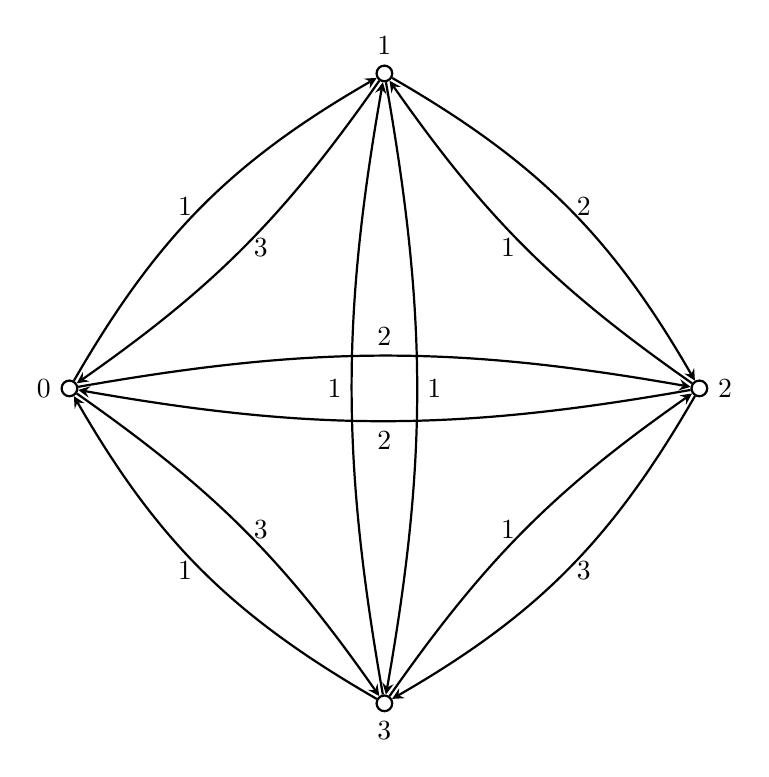
\begin{tikzpicture}
[nodedecorate/.style={shape=circle,inner sep=2pt,draw,thick},%
  arrowdecorate/.style={->,>=stealth,thick}]
% nodes or vertices
\node (0) at (-4,4) [nodedecorate] {};
\node [left] at (0.west) {$0$};
\node (1) at (0,8) [nodedecorate] {};
\node [above] at (1.north) {$1$};
\node (2) at (4,4) [nodedecorate] {};
\node [right] at (2.east) {$2$};
\node (3) at (0,0) [nodedecorate] {};
\node [below] at (3.south) {$3$};
% edges or lines
\path
(0) edge[arrowdecorate,bend left=15] node[left]{$1$} (1)
(0) edge[arrowdecorate,bend left=10] node[above]{$2$} (2)
(0) edge[arrowdecorate,bend left=10] node[right]{$3$} (3)
(1) edge[arrowdecorate,bend left=10] node[right]{$3$} (0)
(1) edge[arrowdecorate,bend left=15] node[right]{$2$} (2)
(1) edge[arrowdecorate,bend left=10] node[right]{$1$} (3)
(2) edge[arrowdecorate,bend left=10] node[below]{$2$} (0)
(2) edge[arrowdecorate,bend left=10] node[left]{$1$} (1)
(2) edge[arrowdecorate,bend left=15] node[right]{$3$} (3)
(3) edge[arrowdecorate,bend left=15] node[left]{$1$} (0)
(3) edge[arrowdecorate,bend left=10] node[left]{$1$} (1)
(3) edge[arrowdecorate,bend left=10] node[left]{$1$} (2);
\end{tikzpicture}
}
\subfigure[]{
\begin{tikzpicture}
[nodedecorate/.style={shape=circle,inner sep=2pt,draw,thick},%
  linedecorate/.style={-,thick}]
% nodes or vertices
\node (0) at (4,-4) [nodedecorate] {};
\node [right] at (0.east) {$0$};
\node (1) at (2,-2) [nodedecorate] {};
\node [right] at (1.east) {$1$};
\node (2) at (6,-6) [nodedecorate] {};
\node [right] at (2.east) {$2$};
\node (3) at (0,0) [nodedecorate] {};
\node [right] at (3.east) {$3$};
% edges or lines
\path
(3) edge[linedecorate] node[left]{$1$} (1)
(1) edge[linedecorate] node[left]{$1$} (0)
(0) edge[linedecorate] node[left]{$2$} (2);
\end{tikzpicture}
}
\caption{Prim's algorithm for digraphs. Above is the original digraph
  and below is the MST produced by Prim's algorithm.}
\label{fig:tree-forests:Prim_algorithm_digraph}
\end{figure}



\begin{center}
\fontsize{9pt}{9pt}
\selectfont
\tt
\begin{lstlisting}
        sage: A = matrix([[0,7,0,5,0,0,0],[0,0,8,9,7,0,0],[0,0,0,0,5,0,0],
         [0,0,0,0,15,6,0],[0,0,0,0,0,8,9],[0,0,0,0,0,0,11],[0,0,0,0,0,0,0]])
        sage: G = Graph(A, format = "adjacency_matrix", weighted = True)
        sage: E = G.edges(); E
        [(0, 1, 7), (0, 3, 5), (1, 2, 8), (1, 3, 9), (1, 4, 7), (2, 4, 5),
         (3, 4, 15), (3, 5, 6), (4, 5, 8), (4, 6, 9), (5, 6, 11)]
        sage: prim(G).edges()
        [(0, 1, 7), (0, 3, 5), (1, 2, 8), (1, 4, 7), (3, 5, 6), (4, 6, 9)]
\end{lstlisting}
\end{center}
%


\begin{figure}[!htbp]
\centering
\subfigure[]{
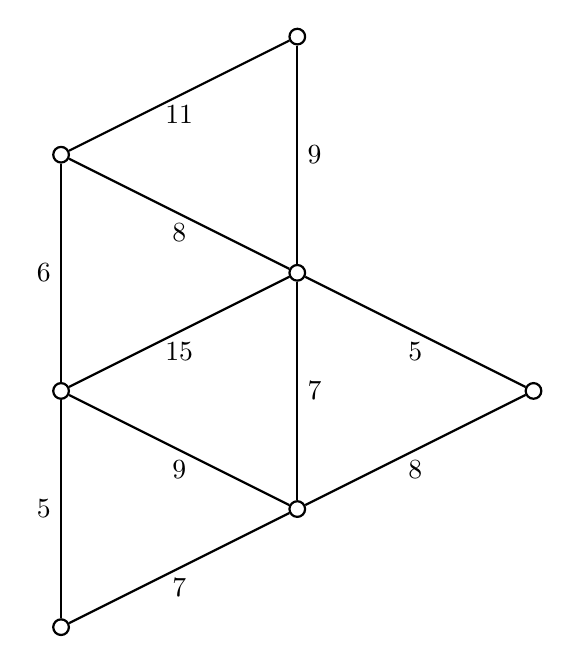
\begin{tikzpicture}
[nodedecorate/.style={shape=circle,inner sep=2pt,draw,thick},%
  linedecorate/.style={-,thick}]
% nodes or vertices
\node (0) at (0,0) [nodedecorate] {};
\node (1) at (3,1.5) [nodedecorate] {};
\node (2) at (6,3) [nodedecorate] {};
\node (3) at (0,3) [nodedecorate] {};
\node (4) at (3,4.5) [nodedecorate] {};
\node (5) at (0,6) [nodedecorate] {};
\node (6) at (3,7.5) [nodedecorate] {};
% edges or lines
\path
(0) edge[linedecorate] node[below]{$7$} (1)
(0) edge[linedecorate] node[left]{$5$} (3)
(1) edge[linedecorate] node[below]{$8$} (2)
(1) edge[linedecorate] node[below]{$9$} (3)
(1) edge[linedecorate] node[right]{$7$} (4)
(2) edge[linedecorate] node[below]{$5$} (4)
(3) edge[linedecorate] node[below]{$15$} (4)
(3) edge[linedecorate] node[left]{$6$} (5)
(4) edge[linedecorate] node[below]{$8$} (5)
(4) edge[linedecorate] node[right]{$9$} (6)
(5) edge[linedecorate] node[below]{$11$} (6);
\end{tikzpicture}
}
\subfigure[]{
\begin{tikzpicture}
[nodedecorate/.style={shape=circle,inner sep=2pt,draw,thick},%
  linedecorate/.style={-,thick}]
% nodes or vertices
\node (6) at (0,0) [nodedecorate] {};
\node [left] at (6.west) {$6$};
\node (4) at (2,2) [nodedecorate] {};
\node [left] at (4.west) {$4$};
\node (1) at (4,4) [nodedecorate] {};
\node [left] at (1.west) {$1$};
\node (2) at (6,2) [nodedecorate] {};
\node [left] at (2.west) {$2$};
\node (0) at (4,6) [nodedecorate] {};
\node [left] at (0.west) {$0$};
\node (3) at (4,8) [nodedecorate] {};
\node [left] at (3.west) {$3$};
\node (5) at (4,10) [nodedecorate] {};
\node [left] at (5.west) {$5$};
% edges or lines
\path
(6) edge[linedecorate] node[below]{$9$} (4)
(4) edge[linedecorate] node[below]{$7$} (1)
(1) edge[linedecorate] node[above]{$8$} (2)
(1) edge[linedecorate] node[right]{$7$} (0)
(0) edge[linedecorate] node[right]{$5$} (3)
(3) edge[linedecorate] node[right]{$6$} (5);
\end{tikzpicture}
}
\caption{Another example of Prim's algorithm. On the left is the
  original graph. On the right is the MST produced by Prim's algorithm.}
\label{fig:tree-forests:Prim_algorithm_digraph2}
\end{figure}


\subsection{Bor\r{u}vka's algorithm}

Bor\r{u}vka's algorithm algorithm is an algorithm
for finding a minimum spanning tree in a connected graph for
which all edge weights are distinct.
\index{Bor\r{u}vka's algorithm}

Pseudocode for Bor\r{u}vka's algorithm is:

\begin{itemize}
\item
Begin with a connected graph G containing edges of distinct
 weights, and an empty set of edges T
\item
While the vertices of G connected by T are disjoint:
\begin{itemize}
\item
Begin with an empty set of edges E
\item
         For each component:
\begin{itemize}
\item
        Begin with an empty set of edges S
\item
        For each vertex in the component:
 \begin{itemize}
\item
Add the cheapest edge from the vertex in
             the component to another vertex in a disjoint component to S
\end{itemize}
        Add the cheapest edge in S to E
\end{itemize}
    Add the resulting set of edges E to T.
\end{itemize}
The resulting set of edges T is the minimum spanning tree of G.
\end{itemize}

\begin{example}

In Figure \ref{fig:tree-forests:Boruvkas-algorithm} , we plot the following example.

\begin{center}
\fontsize{9pt}{9pt}
\selectfont
\tt
\begin{lstlisting}
       sage: A = matrix([[0,1,2,5],[0,0,3,6],[0,0,0,4],[0,0,0,0]])
       sage: G = Graph(A, format = "adjacency_matrix", weighted = True)
       sage: boruvka(G)
\end{lstlisting}
\end{center}
%

\begin{figure}[!htbp]
\centering
\subfigure[]{
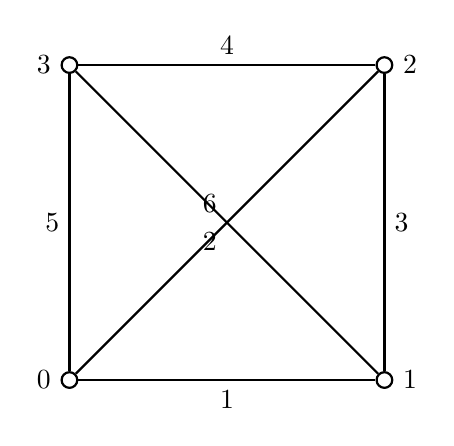
\begin{tikzpicture}
[nodedecorate/.style={shape=circle,inner sep=2pt,draw,thick},%
  linedecorate/.style={-,thick}]
% nodes or vertices
\node (0) at (0,0) [nodedecorate] {};
\node [left] at (0.west) {$0$};
\node (1) at (4,0) [nodedecorate] {};
\node [right] at (1.east) {$1$};
\node (2) at (4,4) [nodedecorate] {};
\node [right] at (2.east) {$2$};
\node (3) at (0,4) [nodedecorate] {};
\node [left] at (3.west) {$3$};
% edges or lines
\path
(0) edge[linedecorate] node[below]{$1$} (1)
(0) edge[linedecorate] node[below left] {$2$} (2)
(0) edge[linedecorate] node[left]{$5$} (3)
(1) edge[linedecorate] node[right]{$3$} (2)
(1) edge[linedecorate] node[above left] {$6$} (3)
(2) edge[linedecorate] node[above]{$4$} (3);
\end{tikzpicture}
}
\qquad
\subfigure[]{
\begin{tikzpicture}
[nodedecorate/.style={shape=circle,inner sep=2pt,draw,thick},%
  linedecorate/.style={-,thick}]
% nodes or vertices
\node (3) at (0,0) [nodedecorate] {};
\node [right] at (3.east) {$3$};
\node (2) at (1,2) [nodedecorate] {};
\node [right] at (2.east) {$2$};
\node (0) at (2,4) [nodedecorate] {};
\node [right] at (0.east) {$0$};
\node (1) at (3,6) [nodedecorate] {};
\node [right] at (1.east) {$1$};
% edges or lines
\path
(3) edge[linedecorate] node[left]{$4$} (2)
(2) edge[linedecorate] node[left]{$2$} (0)
(0) edge[linedecorate] node[left]{$1$} (1);
\end{tikzpicture}
}
\caption{An example of Borovka's algorithm. On the left is the
  original graph. On the right is the MST produced by Boruvka's algorithm.}
\label{fig:tree-forests:Boruvkas-algorithm}
\end{figure}

\end{example}



\begin{center}
\vskip .15in

\begin{Verbatim}[fontsize=\scriptsize,fontfamily=courier,fontshape=tt,frame=single,label=\sage]

def which_index(x,L):
    """
    L is a list of sublists (or tuple of sets or list
    of tuples, etc).

    Returns the index of the first sublist which x belongs
    to, or None if x is not in flatten(L).

    The 0-th element in
    Lx = [L.index(S) for S in L if x in S]
    almost works, but if the list is empty then Lx[0]
    throws an exception.

    EXAMPLES:
        sage: L = [[1,2,3],[4,5],[6,7,8]]
        sage: which_index(3,L)
        0
        sage: which_index(4,L)
        1
        sage: which_index(7,L)
        2
        sage: which_index(9,L)
        sage: which_index(9,L) == None
        True
    """
    for S in L:
        if x in S:
            return L.index(S)
    return None

def boruvka(G):
    """
    Implements Boruvka's algorithm to compute a MST of a graph.

    INPUT:
        G - a connected edge-weighted graph with distinct weights.
    OUTPUT:
        T - a minimum weight spanning tree.

    REFERENCES:
        http://en.wikipedia.org/wiki/Boruvka's_algorithm
    """
    T_vertices = [] # assumes G.vertices = range(n)
    T_edges = []
    T = Graph()
    E = G.edges() # a list of triples
    V = G.vertices()
    # start ugly hack to sort E
    Er = [list(x) for x in E]
    E0 = []
    for x in Er:
        x.reverse()
        E0.append(x)
    E0.sort()
    E = []
    for x in E0:
        x.reverse()
        E.append(tuple(x))
    # end ugly hack to get E is sorted by weight
    for e in E:
        # create about |V|/2 edges of T "cheaply"
        TV = T.vertices()
        if not(e[0] in TV) or not(e[1] in TV):
           T.add_edge(e)
    for e in E:
        # connect the "cheapest" components to get T
        C = T.connected_components_subgraphs()
        VC = [S.vertices() for S in C]
        if not(e in T.edges()) and (which_index(e[0],VC) != which_index(e[1],VC)):
           if T.is_connected():
                break
            T.add_edge(e)
    return T

\end{Verbatim}

\end{center}

Some examples using Sage:


\begin{center}
\fontsize{9pt}{9pt}
\selectfont
\tt
\begin{lstlisting}

        sage: A = matrix([[0,1,2,3],[4,0,5,6],[7,8,0,9],[10,11,12,0]])
        sage: G = DiGraph(A, format = "adjacency_matrix", weighted = True)
        sage: boruvka(G)
        Multi-graph on 4 vertices
        sage: boruvka(G).edges()
        [(0, 1, 1), (0, 2, 2), (0, 3, 3)]
        sage: A = matrix([[0,2,0,5,0,0,0],[0,0,8,9,7,0,0],[0,0,0,0,1,0,0],\
         [0,0,0,0,15,6,0],[0,0,0,0,0,3,4],[0,0,0,0,0,0,11],[0,0,0,0,0,0,0]])
        sage: G = Graph(A, format = "adjacency_matrix", weighted = True)
        sage: E = G.edges(); E
        [(0, 1, 2), (0, 3, 5), (1, 2, 8), (1, 3, 9), (1, 4, 7),
         (2, 4, 1), (3, 4, 15), (3, 5, 6), (4, 5, 3), (4,6, 4), (5, 6, 11)]
        sage: boruvka(G)
        Multi-graph on 7 vertices
        sage: boruvka(G).edges()
        [(0, 1, 2), (0, 3, 5), (2, 4, 1), (3, 5, 6), (4, 5, 3), (4, 6, 4)]
        sage: A = matrix([[0,1,2,5],[0,0,3,6],[0,0,0,4],[0,0,0,0]])
        sage: G = Graph(A, format = "adjacency_matrix", weighted = True)
        sage: boruvka(G).edges()
        [(0, 1, 1), (0, 2, 2), (2, 3, 4)]
        sage: A = matrix([[0,1,5,0,4],[0,0,0,0,3],[0,0,0,2,0],[0,0,0,0,0],[0,0,0,0,0]])
        sage: G = Graph(A, format = "adjacency_matrix", weighted = True)
        sage: boruvka(G).edges()
        [(0, 1, 1), (0, 2, 5), (1, 4, 3), (2, 3, 2)]

\end{lstlisting}
\end{center}
%

%%-----------------------------------------------------------------------%%
%%--- Binary trees ------------------------------------------------------%%

\section{Binary trees}

See section~3.3 of Gross and Yellen~\cite{GrossYellen1999}.

A binary tree is a rooted tree with at most 2 children per parent.

In this section, we consider

\begin{itemize}
\item binary codes,

\item Gray codes, and

\item Huffman codes.
\end{itemize}

\subsection{Binary codes}


\subsubsection{What is a code?}

A {\it code} is a rule for converting data in one
\index{code}
\index{codeword}
\index{alphabet}
format, or well-defined tangible representation,
into sequences of symbols in another format (and the finite set of symbols
used is called the {\it alphabet}). We shall identify a code
as a finite set of symbols which are the image
of the alphabet under this conversion rule. The elements of this set
are referred to as {\it codewords}. For example, using the ASCII code,
the letters in the English alphabet get converted into numbers
$\{0, 1, \dots, 255\}$. If these numbers are written in binary
then each codeword of a letter has length 8. In this way, we can
reformat, or encode, a ``string'' into a sequence of binary symbols (i.e.,
$0$'s and $1$'s).
{\it Encoding} is the conversion process one way.
{\it Decoding} is the reverse
\index{encode}
\index{decode}
process, converting these sequences of code-symbols back into information
in the original format.


Codes are used for

\begin{itemize}
\item
{\it Economy}. Sometimes this is called ``entropy encoding''
since there is an entropy function which describes how much information
a channel (with a given error rate) can carry and such
codes are designed to maximize entropy as best as possible.
In this case, in addition to simply being given an alphabet $A$, one
might be given a ``weighted alphabet,'' i.e., an alphabet for which each
symbol $a\in A$ is associated with a non-negative number
$w_a\geq 0$ (in practice, the probability that the
symbol $a$ occurs in a typical word).

\item
{\it Reliability}. Such codes are called ``error-correcting codes,''
since such codes are designed to communicate information
over a noisy channel in such a way that the errors in transmission are
likely to be correctable.

\item
{\it Security}. Such codes ae called ``cryptosystems.''
In this case, the inverse of the coding function $c:A\to B^*$ is designed to be
computationally infeasible. In other words, the coding function
$c$ is designed to be a ``trapdoor function.''

\end{itemize}

Other codes are merely simpler ways to communicate information
(flag semaphores, color codes, genetic codes, braille codes, musical scores, chess
notation, football diagrams, and so on), and have little or no
mathematical structure. We shall not study them.



\subsubsection{Basic definitions}

If every word in the code has the same length, the code is called
a {\it block code}. If a code is not a block code then it is called
a {\it variable-length} code.
\index{code!block}
\index{code!variable-length}
A {\it prefix-free} code is a code (typically one of variable-length)
with the property that there is no valid codeword in the code that
is a prefix (start) of any other codeword\footnote{In other words,
a codeword $s=s_1 \dots s_m$ is a {\it prefix} of a codeword
$t=t_1\dots t_n$ if and only if $m\leq n$ and
$s_1=t_1$, \dots, $s_m=t_m$. Codes which are prefix-free are easier
to decode than codes which are not prefix-free.}.
This is the {\it prefix-free condition}.
\index{code!prefix-free}

One example of a prefix-free code is the ASCII code.
Another example is

\[
00, 01, 100.
\]
On the other hand, a non-example is the code

\[
00, 01, 010, 100
\]
since the second codeword is a prefix of the third one.
Another non-example is Morse code recalled in
Table~\ref{tab:trees_forests:Morse_code} (we use $0$ for
$\cdot$ (``dit'') and $1$ for $-$ (``dah'')).
\index{code!Morse}

\begin{table}[!htbp]
\centering
\begin{tabular}{|c|c||c|c|} \hline
A & 01    & N & 10 \\
B & 1000  & O & 111 \\
C & 1010  & P & 0110 \\
D & 100   & Q & 1101 \\
E & 0     & R & 010 \\
F & 0010  & S & 000 \\
G & 110   & T & 1 \\
H & 0000  & U & 001 \\
I & 00    & V & 0001 \\
J & 0111  & W & 011 \\
K & 101   & X & 1001 \\
L & 0100  & Y & 1011 \\
M & 11    & Z & 1100 \\\hline
\end{tabular}
\caption{Morse code}
\label{tab:trees_forests:Morse_code}
\end{table}

For example, look at the Morse code for {\tt a} and the Morse code for
{\tt w}. These codewords violate the prefix-free condition.

\subsubsection{Gray codes}

History\footnote{This
history comes from an unpublished section 7.2.1.1
(``Generating all $n$-tuples'')
in volume 4 of Donald Knuth's {\bf The Art of Computer Programming}.
}
: Frank Gray (1887-1969) wrote about the so-called Gray codes in a
1951 paper published in the Bell System Technical Journal,
and then patented a device (used for television sets)
based on it in 1953. However, the idea of a binary Gray code
appeared earlier. In fact, it appeared in an earlier patent
(one by Stibitz in 1943). It was also used in E. Baudot's
(a French engineer) telegraph machine of 1878 and in
a French booklet by L. Gros on the solution to the
``Chinese ring puzzle'' published in 1872.

The term ``Gray code'' is ambiguous. It is actually a
large family of sequences of $n$-tuples. Let
${\mathbb{Z}}_m=\{0,1,\dots,m-1\}$. More precisely, an
{\it $m$-ary Gray code of length $n$} (called a {\it binary
Gray code} when $m=2$) is a sequence of
all possible (namely, $N=m^n$) $n$-tuples
\index{Gray code!binary}
\index{Gray code!$m$-ary}

\[
g_1,g_2,\dots, g_N,
\]
where
\begin{itemize}
\item
each $g_i\in {\mathbb{Z}}_m^n$,
\item
$g_i$ and $g_{i+1}$ differ by $1$ in exactly one
coordinate.
\end{itemize}
In other words, an $m$-ary Gray code of length
$n$ is a particular way to order the set of all
$m^n$ $n$-tuples whose coordinates are taken from
${\mathbb{Z}}_m$. From the transmission/communication
perspective, this sequence has two advantages:

\begin{itemize}
\item
It is easy and fast to produce the sequence, since
successive entries differ in only one coordinate.

\item
An error is relatively easy to detect, since you can
compare an $n$-tuple with the previous one. If they
difer in more than one coordinate, you know an error
was made.

\end{itemize}

\begin{example}
{\rm
Here is a $3$-ary Gray code of length $2$:

\[
[0, 0], [1, 0], [2, 0], [2, 1], [1, 1], [0, 1], [0, 2], [1, 2], [2, 2]
\]
and here is a binary Gray code of length $3$:

\[
[0, 0, 0], [1, 0, 0], [1, 1, 0], [0, 1, 0], [0, 1, 1], [1, 1, 1], [1, 0, 1], [0, 0, 1].
\]
}
\end{example}

Gray codes have applications to engineering,
recreational mathematics (solving the Tower of Hanoi
puzzle, ``The Brain'' puzzle, the ``Chinese ring puzzle'',
and others), and to mathematics (for example, aspects of
combinatorics, computational group theory
and the computational aspects of linear codes).

\subsubsection{Binary Gray codes}

Consider the so-called $n$-hypercube graph
$Q_n$. This can be envisioned as the graph whose
vertices are the vertices of a cube in
$n$-space
\index{graph!hypercube}

\[
\{(x_1,\dots,x_n)\ |\ 0\leq x_i\leq 1\},
\]
and whose edges are those line segments in
${\mathbb{R}}^n$ connecting two ``neighboring''
vertices (namely, two vertices which differ
in exactly one coordinate).
A binary Gray code of length $n$ can be regarded as a
path on the hypercube graph $Q_n$ which visits
each vertex of the cube exactly once.
In other words, a binary Gray code of length $n$
may be identified with a
Hamiltonian cycle on the graph $Q_n$
(see Figure \ref{fig:trees_forests:gray_code_cube} for an example).

\begin{figure}[!htbp]
\centering
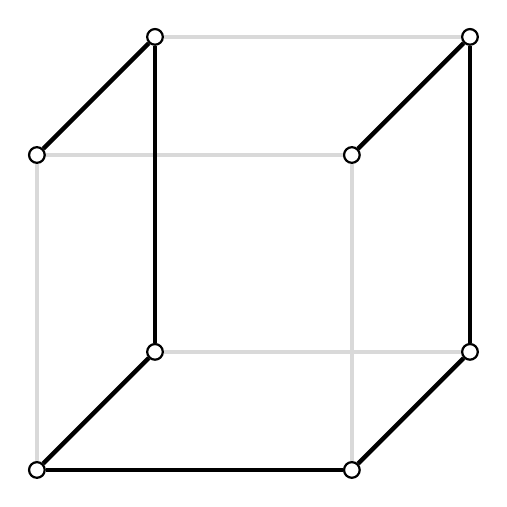
\begin{tikzpicture}
[nodedecorate/.style={shape=circle,inner sep=2pt,draw,thick},%
  darkline/.style={-,ultra thick},
  lightline/.style={-,ultra thick,color=gray!30}]
% nodes or vertices
% foreground square
\node (1) at (0,0) [nodedecorate] {};
\node (2) at (4,0) [nodedecorate] {};
\node (3) at (4,4) [nodedecorate] {};
\node (4) at (0,4) [nodedecorate] {};
% background square
\node (5) at (1.5,1.5) [nodedecorate] {};
\node (6) at (5.5,1.5) [nodedecorate] {};
\node (7) at (5.5,5.5) [nodedecorate] {};
\node (8) at (1.5,5.5) [nodedecorate] {};
% edges or lines
\path
% foreground square
(1) edge[darkline] node {} (2)
(2) edge[lightline] node {} (3)
(3) edge[lightline] node {} (4)
(4) edge[lightline] node {} (1)
% background square
(5) edge[lightline] node {} (6)
(6) edge[darkline] node {} (7)
(7) edge[lightline] node {} (8)
(8) edge[darkline] node {} (5)
% joining foreground and background squares
(1) edge[darkline] node {} (5)
(2) edge[darkline] node {} (6)
(3) edge[darkline] node {} (7)
(4) edge[darkline] node {} (8);
\end{tikzpicture}
\caption{Viewing $\Gamma_3$ as a Hamiltonian path on $Q_3$.}
\label{fig:trees_forests:gray_code_cube}
\end{figure}


How do you efficiently compute a Gray code?

Perhaps the simplest way to state the idea of
quickly constructing
the {\it reflected binary Gray code} $\Gamma_n$
of length $n$ is as follows:

\[
\Gamma_0=[],\ \ \ \
\Gamma_{n}=[0,\Gamma_{n-1}],[1,\Gamma_{n-1}^{rev}],
\]
where $\Gamma_m^{rev}$ means the Gray code in
reverse order. For instance, we have

\[
\Gamma_0=[],
\]
\[
\Gamma_1 = [0], [1],
\]
\[
\Gamma_2=[[0,0],[0,1],[1,1],[1,0],
\]
and so on. This is a nice procedure if you want to create
the entire list at once (which, by the way, gets very long
very fast).

An implementation of the reflected Gray code using Python is given below.

\begin{Verbatim}[fontsize=\scriptsize,fontfamily=courier,fontshape=tt,frame=single,label=Python
  3.0]

def graycode(length,modulus):
    """
    Returns the n-tuple reflected Gray code mod m.


    EXAMPLES:
        sage: graycode(2,4)

        [[0, 0],
         [1, 0],
         [2, 0],
         [3, 0],
         [3, 1],
         [2, 1],
         [1, 1],
         [0, 1],
         [0, 2],
         [1, 2],
         [2, 2],
         [3, 2],
         [3, 3],
         [2, 3],
         [1, 3],
         [0, 3]]

    """
    n,m = length,modulus
    F = range(m)
    if n == 1:
        return [[i] for i in F]
    L = graycode(n-1, m)
    M = []
    for j in F:
        M = M+[ll+[j] for ll in L]
    k = len(M)
    Mr = [0]*m
    for i in range(m-1):
        i1 = i*int(k/m)       # this requires Python 3.0 or Sage
        i2 = (i+1)*int(k/m)
        Mr[i] = M[i1:i2]
    Mr[m-1] = M[(m-1)*int(k/m):]
    for i in range(m):
        if is_odd(i):
            Mr[i].reverse()
    M0 = []
    for i in range(m):
        M0 = M0+Mr[i]
    return M0

\end{Verbatim}

\vskip .2in
Consider the reflected binary code
of length $8$, $\Gamma_8$. This has $2^8=256$ codewords.
\sage can easily create the list plot of the coordinates
$(x,y)$, where $x$ is an integer $j \in {\mathbb{Z}}_{256}$
which indexes the codewords in $\Gamma_8$
and the corresponding $y$ is the $j$-th
codeword in $\Gamma_8$ converted to decimal.
This will give us some idea of how the Gray code
``looks'' in some sense. The plot is given in Figure \ref{fig:Gamma8}.

%% Figure created using the following code.
%% def int2binary(m, n):
%%    '''
%%    returns GF(2) vector of length n obtained
%%    from the binary repr of m, padded by 0's
%%    (on the left) to length n.
%%
%%    EXAMPLES:
%%        sage: for j in range(8):
%%        ....:     print int2binary(j,3)+int2binary(int(j/2),3)
%%        ....:
%%        (0, 0, 0)
%%        (0, 0, 1)
%%        (0, 1, 1)
%%        (0, 1, 0)
%%        (1, 1, 0)
%%        (1, 1, 1)
%%        (1, 0, 1)
%%        (1, 0, 0)
%%    '''
%%    s = bin(m)
%%    k = len(s)
%%    F = GF(2)
%%    b = [F(0)]*n
%%    for i in range(2,k):
%%        b[n-k+i] = F(int(s[i]))
%%    return vector(b)
%%
%% def binary2int(b):
%%    "''
%%    inverts int2binary
%%
%%    "''
%%    k = len(b)
%%    n = sum([int(b[i])*2**(k-1-i) for i in range(k)])
%%    return n
%%
%% def graycodeword(m, n):
%%    '''
%%    returns the mth codeword in the reflected binary Gray code
%%    of length n.
%%
%%    EXAMPLES:
%%        sage: graycodeword(3,3)
%%        (0, 1, 0)
%%    '''
%%    return int2binary(m,n)+int2binary(int(m/2),n)
%%
%% sage: L = [(k,binary2int(graycodeword(k, 8))) for k in range(256)]
%% sage: P = list_plot(L); P.save(``gray-code-2-8.png'')
\begin{figure}[!htbp]
\centering
\includegraphics{image/graycode-gamma8}
\caption{List plot of $\Gamma_8$ created using Sage.}
\label{}
\end{figure}

What if you only want to compute the
$i$-th Gray codeword in the Gray code of length $n$?
Can it be computed quickly as well without computing the
entire list?
At least in the case of the reflected binary Gray code, there
is a very simple way to do this. The $k$-th element in the
above-described reflected binary Gray code of length $n$
is obtained by simply adding the binary representation of
$k$ to the binary representation of the integer part of
$k/2$.

An example using \sage is given below.

\begin{Verbatim}[fontsize=\scriptsize,fontfamily=courier,fontshape=tt,frame=single,label=\sage]

def int2binary(m, n):
    '''
    returns GF(2) vector of length n obtained
    from the binary repr of m, padded by 0's
    (on the left) to length n.

    EXAMPLES:
        sage: for j in range(8):
        ....:     print int2binary(j,3)+int2binary(int(j/2),3)
        ....:
        (0, 0, 0)
        (0, 0, 1)
        (0, 1, 1)
        (0, 1, 0)
        (1, 1, 0)
        (1, 1, 1)
        (1, 0, 1)
        (1, 0, 0)
    '''
    s = bin(m)
    k = len(s)
    F = GF(2)
    b = [F(0)]*n
    for i in range(2,k):
        b[n-k+i] = F(int(s[i]))
    return vector(b)

def graycodeword(m, n):
    '''
    returns the kth codeword in the reflected binary Gray code
    of length n.

    EXAMPLES:
        sage: graycodeword(3,3)
        (0, 1, 0)
    '''
    return int2binary(m,n)+int2binary(int(m/2),n)

\end{Verbatim}

\begin{exercise}
Convert the above function {\tt graycodeword} into a pure Python
function.
\end{exercise}


%%-----------------------------------------------------------------------%%
%%--- Huffman codes -----------------------------------------------------%%

\section{Huffman codes}
\label{sec:trees_forests:Huffman_codes}

An \emph{alphabet}\index{alphabet} $A$ is a finite set whose elements
are referred to as \emph{symbols}. A \emph{word}\index{word} (or
\emph{string}\index{string} or \emph{message}\index{message}) over $A$
is a finite sequence of symbols in $A$ and the \emph{length} of the
word is the number of symbols it contains. A word is usually written
by concatenating symbols together: $a_1 a_2 \cdots a_k$ ($a_i \in A$)
is a word of length $k$.

A commonly occurring alphabet in practice is the \emph{binary alphabet}
$\{0,1\}$. A word over the binary alphabet is a finite sequence of
$0$'s and $1$'s. If $A$ is an alphabet, let $A^*$ denote the set of
all words in $A$. The length of a word is denoted by vertical
bars. That is, if $w = a_1 \cdots a_k$ is a word over $A$, then define
$|w|: A^* \longrightarrow \ZZ$ by
\[
|w|
=
|a_1 \cdots a_k|
=
k.
\]
Let $A$ and $B$ be two alphabets. A \emph{code}\index{code} for $A$
using $B$ is an injection $c: A \longrightarrow B^*$. By abuse of
notation, we often denote the code simply by the set
\[
C
=
c(A)
=
\{c(a) \;|\; a \in A\}.
\]
The elements of $C$ are called \emph{codewords}\index{codeword}. If
$B$ is the binary alphabet, then $C$ is called a
\emph{binary code}\index{code!binary}.


%%--- Tree representation -----------------------------------------------%%

\subsection{Tree representation}

Any binary code can be represented by a tree, as
Example~\ref{eg:tree_forests:binary_code_tree_representation} shows.

\begin{example}
\label{eg:tree_forests:binary_code_tree_representation}
Let $\BB_\ell$ be the binary code of length $\leq \ell$. Represent
codewords of $\BB_\ell$ using trees.
\end{example}

\begin{proof}[Solution]
Here is how to represent the code $\BB_\ell$ consisting of all binary
strings of length $\leq \ell$. Start with the
\emph{root node}\index{node!root} $\varepsilon$\index{$\varepsilon$}
being the empty string. The two children of this node, $v_0$ and
$v_1$, correspond to the two strings of length $1$. Label $v_0$ with a
``$0$'' and $v_1$ with a ``$1$''. The two children of $v_0$,
i.e. $v_{00}$ and $v_{01}$, correspond to the strings of length $2$
which start with a $0$. Similarly, the  two children of $v_1$,
i.e. $v_{10}$ and $v_{11}$, correspond to the strings of length $2$
that each starts with a $1$. Continue creating child nodes until we
reach length $\ell$, at which point we stop. There are a total of
$2^{\ell + 1} - 1$ nodes in this tree and $2^\ell$ of them are
\emph{leaves}\index{leaf}~(vertices of a tree with degree $1$,
i.e. childless nodes). Note that the parent of any node is a prefix to
that node. Label each node $v_s$ with the string ``$s$'', where $s$ is
a binary sequence of length $\leq \ell$. See
Figure~\ref{fig:trees_forests:tree_representation_B_2} for an example
when $\ell = 2$.
\end{proof}

\begin{figure}[!htbp]
\centering
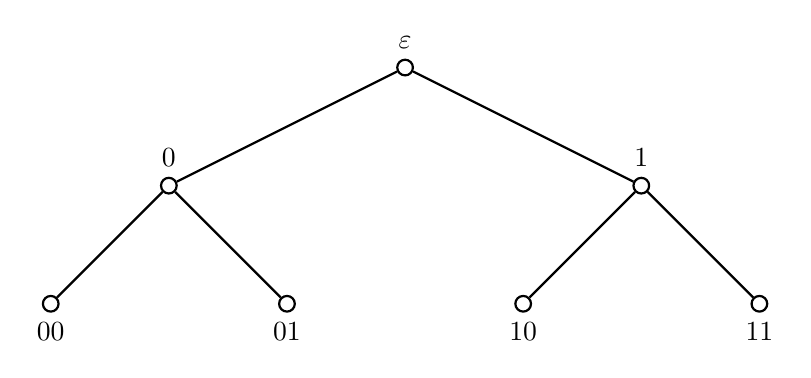
\begin{tikzpicture}
[nodedecorate/.style={shape=circle,inner sep=2pt,draw,thick},%
  linedecorate/.style={-,thick},%
  scale=1.5]
%% nodes or vertices
\foreach \nodename/\x/\y/\direction/\navigate in {
  00/0/0/below/south, 01/2/0/below/south, 10/4/0/below/south,
  11/6/0/below/south, 0/1/1/above/north, 1/5/1/above/north} {
  \node (\nodename) at (\x,\y) [nodedecorate] {};
  \node [\direction] at (\nodename.\navigate) {$\nodename$};
}
\node (e) at (3,2) [nodedecorate] {};
\node [above] at (e.north) {$\varepsilon$};
%% edges or lines
\path
\foreach \startnode/\endnode in {0/00, 0/01, 1/10, 1/11, e/0, e/1} {
  (\startnode) edge[linedecorate] node {} (\endnode)
};
\end{tikzpicture}
\caption{Tree representation of the binary code $\BB_2$.}
\label{fig:trees_forests:tree_representation_B_2}
\end{figure}

In general, if $C$ is a code contained in $\BB_\ell$, then to create
the tree for $C$, start with the tree for $\BB_\ell$. First, remove
all nodes associated to a binary string for which it and all of its
descendents are not in $C$. Next, remove all labels which do not
correspond to codewords in $C$. The resulting labeled graph is the
tree associated to the binary code $C$.
\index{code!tree}

For visualizing the construction of Huffman codes later, it is
important to see that one can \emph{reverse} this construction to
start from such a binary tree and recover a binary code from it. The
codewords are determined by the following rules:
%
\begin{itemize}
\item The root node gets the empty codeword.

\item Each left-ward branch gets a $0$ appended to the end of its
  parent. Each right-ward branch gets a $1$ appended to the end.
\end{itemize}


%%--- Uniquely decodable codes ------------------------------------------%%

\subsection{Uniquely decodable codes}

If $c: A \longrightarrow B^*$ is a code, then we can extend $c$ to
$A^*$ by \emph{concatenation}:
\[
c(a_1 a_2 \cdots a_k)
=
c(a_1) c(a_2) \cdots c(a_k).
\]
If the extension $c: A^* \longrightarrow T^*$ is also an injection,
then $c$ is called \emph{uniquely decodable}.
\index{code!uniquely decodable}

\begin{example}
Is the Morse code\index{code!Morse} in
Table~\ref{tab:trees_forests:Morse_code} uniquely decodable? Why or
why not?
\end{example}

\begin{proof}[Solution]
Note that these Morse codewords all have lengths less than or equal to
$4$. Other commonly occurring symbols used~(the digits $0$ through
$9$, punctuation symbols, and some others) are also encodable in Morse
code, but they use longer codewords.

Let $A$ denote the English alphabet, $B = \{0, 1\}$ the binary
alphabet, and $C: A \longrightarrow B^*$ the Morse code. Since
$c(ET) = 01 = c(A)$, it is clear that the Morse code is \emph{not}
uniquely decodable.
\end{proof}

In fact, prefix-free implies uniquely decodable.

\begin{theorem}
If a code $c: A \longrightarrow B^*$ is prefix-free, then it is
uniquely decodable.
\end{theorem}

\begin{proof}
We use induction on the length of a message. We want to show that if
$x_1 \cdots x_k$ and $y_1 \cdots y_\ell$ are messages with
$c(x_1) \cdots c(x_k) = c(y_1) \cdots c(y_\ell)$, then
$x_1 \cdots x_k = y_1 \cdots y_\ell$. This in turn implies $k = \ell$
and $x_i = y_i$ for all $i$.

The case of length $1$ follows from the fact that
$c: A \longrightarrow B^*$ is injective~(by the definition of a
code).

Suppose that the statement of the theorem holds for all
codes of length $< m$. We must show that the length $m$ case is
true. Suppose $c(x_1) \cdots c(x_k) = c(y_1) \cdots c(y_\ell)$, where
$m = \max(k, \ell)$. These strings are equal, so the substring
$c(x_1)$ of the left-hand side and the substring $c(y_1)$ of the
right-hand side are either equal or one is contained in the other. If,
say, $c(x_1)$ is properly contained in $c(y_1)$, then $c$ is not
prefix-free. Likewise if $c(y_1)$ is properly contained in
$c(x_1)$. Therefore, $c(x_1) = c(y_1)$, which implies $x_1 = y_1$. Now
remove this codeword from both sides, so
$c(x_2) \cdots c(x_k) = c(y_2) \cdots c(y_\ell)$. By the induction
hypothesis, $x_2 \cdots x_k = y_2 \cdots y_\ell$. These facts together
imply $k = \ell$ and $x_i = y_i$ for all $i$.
\end{proof}

Consider now a weighted alphabet $(A,p)$, where
$p: A \longrightarrow [0,1]$ satisfies $\sum_{a \in A}p(a) = 1$, and a
code $c: A \longrightarrow B^*$. In other words, $p$ is a probability
distribution on $A$. Think of $p(a)$ as the probability that the
symbol $a$ arises in an typical message. The
\emph{average word length} $L(c)$ is\footnote{
  In probability terminology, this is the expected value $E(X)$ of the
  random variable $X$ which assigns to a randomly selected symbol in
  $A$, the length of the associated codeword in $C$.
}
\[
L(c)
=
\sum_{a \in A} p(a) \cdot |c(a)|
\]
where $|\cdot|$ denotes the \emph{length} of a codeword.
\index{length of codeword}
Given a weighted alphabet $(A,p)$ as above, a code
$c: A \longrightarrow B^*$ is called \emph{optimal} if there is no
such code with a smaller average word length.
\index{code!optimal}
Optimal codes satisfy the following amazing property. For a proof,
which is very easy and highly recommended for anyone who is curious to
see more, refer to section~3.6 of Biggs~\cite{Biggs2009}.

\begin{lemma}
\label{lem:trees_forests:binary_optimal_prefix_free_code}
Suppose $c: A \longrightarrow B^*$ is a binary optimal prefix-free
code and let $\ell = \max_{a \in A} \big(|c(a)|\big)$ denote the
maximum length of a codeword. The following statements hold.
%
\begin{enumerate}
\item If $|c(a')|>|c(a)|$, then $p(a')\leq p(a)$.

\item The subset of codewords of length $\ell$,
\[
C_\ell
=
\{c \in c(A) \;|\; \ell = |c(a)|\},
\]
contains two codewords of the form $b0$ and $b1$ for some $b \in B^*$.
\end{enumerate}
\end{lemma}


%%--- Huffman coding ----------------------------------------------------%%

\subsection{Huffman coding}

The Huffman code construction is based on the second property in
Lemma~\ref{lem:trees_forests:binary_optimal_prefix_free_code}. Using
this property, in 1952 David Huffman~\cite{Huffman1952} presented an
optimal prefix-free binary code, which has since been named Huffman
code.

Here is the recursive/inductive construction of a Huffman code. We
shall regard the binary Huffman code as a tree, as described
above. Suppose that the weighted alphabet $(A,p)$ has $n$ symbols. We
assume inductively that there is an optimal prefix-free binary code
for any weighted alphabet $(A',p')$ having $<n$ symbols.

\begin{description}
\item[Huffman's rule 1] Let $a,a' \in A$ be symbols with the smallest
  weights. Construct a new weighted alphabet with $a,a'$ replaced by
  the single symbol $a^* = aa'$ and having weight
  $p(a^*) = p(a) + p(a')$. All other symbols and weights remain
  unchanged.

\item[Huffman's rule 2] For the code $(A',p')$ above, if $a^*$ is
  encoded as the binary string $s$, then the encoded binary string for
  $a$ is $s0$ and the encoded binary string for $a'$ is $s1$.
\end{description}

The above two rules tell us how to inductively build the tree
representation for the Huffman code of $(A,p)$ up from its
leaves~(associated to the low weight symbols).
%
\begin{itemize}
\item Find two different symbols of lowest weight, $a$ and $a'$. If
  two such symbols do not exist, stop. Replace the weighted alphabet
  with the new weighted alphabet as in Huffman's rule 1.

\item Add two nodes~(labeled with $a$ and $a'$, respectively) to the
  tree, with parent $a^*$ (see Huffman's rule 1).

\item If there are no remaining symbols in $A$, label the parent $a^*$
  with the empty set and stop. Otherwise, go to the first step.
\end{itemize}

These ideas are captured in
Algorithm~\ref{alg:trees_forests:binary_tree_Huffman_codes}, which
outlines steps to construct a binary tree corresponding to the Huffman
code of an alphabet.
Line~\ref{alg:Huffman_tree:initialize_priority_queue} initializes a
minimum priority queue $Q$ with the symbols in the alphabet $A$.
Line~\ref{alg:Huffman_tree:empty_binary_tree} creates an empty binary
tree that will be used to represent the Huffman code corresponding to
$A$. The for loop from lines~\ref{alg:Huffman_tree:for_loop:start}
to~\ref{alg:Huffman_tree:insert_into_queue} repeatedly extracts from
$Q$ two elements $a$ and $b$ of minimum weights. We then create a new
vertex $z$ for the tree $T$ and also let $a$ and $b$ be vertices of
$T$. The weight $W[z]$ of $z$ is the sum of the weights of $a$ and
$b$. We let $z$ be the parent of $a$ and $b$, and insert the new edges
$za$ and $zb$ into $T$. The newly created vertex $z$ is now inserted
into $Q$ with priority $W[z]$. After $n - 1$ rounds of the for loop,
the priority queue has only one element in it, namely the root $r$ of
the binary tree $T$. We extract $r$ from
$Q$~(line~\ref{alg:Huffman_tree:extract_tree_root}) and return it
together with $T$~(line~\ref{alg:Huffman_tree:return_tree_and_root}).

\begin{algorithm}[!htpb]
\dontprintsemicolon  % no semicolon at end of pseudocode statements
%% data section
\SetKwInOut{Input}{Input}
\SetKwInOut{Output}{Output}
%% input/output
\Input{An alphabet $A$ of $n$ symbols. A weight list $W$ of size $n$
  such that $W[i]$ is the weight of $a_i \in A$.}
\Output{A binary tree $T$ representing the Huffman code of $A$ and the
  root $r$ of $T$.}
\BlankLine
%% algorithm body
$n \leftarrow |A|$\;
$Q \leftarrow A$~\nllabel{alg:Huffman_tree:initialize_priority_queue}~\tcc*[f]{minimum priority queue}\;
$T \leftarrow \text{empty tree}$~\nllabel{alg:Huffman_tree:empty_binary_tree}\;
\For{$i \leftarrow 1, 2, \dots, n-1$~\nllabel{alg:Huffman_tree:for_loop:start}}{
  $a \leftarrow \extractMin(Q)$\;
  $b \leftarrow \extractMin(Q)$\;
  $z \leftarrow$ node with left child $a$ and right child $b$\;
  add the edges $za$ and $zb$ to $T$\;
  $W[z] \leftarrow W[a] + W[b]$\;
  insert $z$ into priority queue $Q$~\nllabel{alg:Huffman_tree:insert_into_queue}\;
}
$r \leftarrow \extractMin(Q)$~\nllabel{alg:Huffman_tree:extract_tree_root}\;
\Return $(T, r)$~\nllabel{alg:Huffman_tree:return_tree_and_root}\;
\caption{Binary tree representation of Huffman codes.}
\label{alg:trees_forests:binary_tree_Huffman_codes}
\end{algorithm}

The running time analysis of
Algorithm~\ref{alg:trees_forests:binary_tree_Huffman_codes} depends on
the implementation of the priority queue $Q$. Suppose $Q$ is a simple
unsorted list. The initialization on
line~\ref{alg:Huffman_tree:initialize_priority_queue} requires $O(n)$
time. The for loop from line~\ref{alg:Huffman_tree:for_loop:start}
to~\ref{alg:Huffman_tree:insert_into_queue} is executed exactly
$n - 1$ times. Searching $Q$ to determine the element of minimum
weight requires time at most $O(n)$. Determining two elements of
minimum weights requires time $O(2n)$. The for loop requires time
$O(2n^2)$, which is also the time requirement for the algorithm. An
efficient implementation of the priority queue $Q$, e.g. as a binary
minimum heap, can lower the running time of
Algorithm~\ref{alg:trees_forests:binary_tree_Huffman_codes} down to
$O(n \log_2(n))$.

Algorithm~\ref{alg:trees_forests:binary_tree_Huffman_codes} represents
the Huffman code of an alphabet as a binary tree $T$ rooted at $r$. To
determine the actual encoding of each symbol in the alphabet, we feed
$T$ and $r$ to
Algorithm~\ref{alg:trees_forests:Huffman_encoding_alphabet} to obtain
the encoding of each symbol. Starting from the root $r$ whose
designated label is the empty string $\varepsilon$, the algorithm
traverses the vertices of $T$ in a breadth-first search fashion. If
$v$ is an internal vertex with label \verb!e!, the label of its left
child is the concatenation \verb!e0! and for the rigth child of $v$ we
assign the label \verb!e1!. If $v$ happens to be a leaf vertex, we
take its label to be its Huffman encoding. Any Huffman encoding
assigned to a symbol of an alphabet is not unique. Either of the two
children of an internal vertex can be designated as the left
(resp. right) vertex. The running time of
Algorithm~\ref{alg:trees_forests:Huffman_encoding_alphabet} is
$O(|V|)$, where $V$ is the vertex set of $T$.

\begin{algorithm}[!htpb]
\dontprintsemicolon  % no semicolon at end of pseudocode statements
%% data section
\SetKwInOut{Input}{Input}
\SetKwInOut{Output}{Output}
\SetKwData{treeRoot}{root}
\SetKwData{one}{1}
\SetKwData{zero}{0}
%% input/output
\Input{A binary tree $T$ representing the Huffman code of an alphabet
  $A$. The root $r$ of $T$.}
\Output{A list $H$ representing a Huffman code of $A$, where $H[a_i]$
  corresponds to a Huffman encoding of $a_i \in A$.}
\BlankLine
%% algorithm body
$H \leftarrow [\,]$~\tcc*[f]{list of Huffman encodings}\;
$Q \leftarrow [r]$~\tcc*[f]{queue of vertices}\;
\While{$\length(Q) > 0$}{
  $\treeRoot \leftarrow \dequeue(Q)$\;
  \eIf{\treeRoot \emph{is a leaf}}{
    $H[\treeRoot] \leftarrow$ label of \treeRoot\;
  }{
    $a \leftarrow$ left child of \treeRoot\;
    $b \leftarrow$ right child of \treeRoot\;
    $\enqueue(Q, a)$\;
    $\enqueue(Q, b)$\;
    label of $a \leftarrow$ label of \treeRoot $+$ \zero\;
    label of $b \leftarrow$ label of \treeRoot $+$ \one\;
  }
}
\Return $H$\;
\caption{Huffman encoding of an alphabet.}
\label{alg:trees_forests:Huffman_encoding_alphabet}
\end{algorithm}

\begin{example}
Consider the alphabet $A = \{a, b, c, d, e, f\}$ with corresponding
weights $w(a) = 19$, $w(b) = 2$, $w(c) = 40$, $w(d) = 25$,
$w(e) = 31$, and $w(f) = 3$. Construct a binary tree representation of
the Huffman code of $A$ and determine the encoding of each symbol of
$A$.
\end{example}

\begin{proof}[Solution]
Use Algorithm~\ref{alg:trees_forests:binary_tree_Huffman_codes} to
construct a binary tree representation of the weighted alphabet
$A$. The resulting binary tree $T$ is shown in
Figure~\ref{fig:trees_forests:eg:binary_tree_Huffman_encodings:binary_tree},
where $a_i: w_i$ is an abbreviation for ``vertex $a_i$ has weight
$w_i$.'' The binary tree is rooted at $k$. To encode each alphabetic
symbol, input $T$ and $k$ into
Algorithm~\ref{alg:trees_forests:Huffman_encoding_alphabet} to get the
encodings shown in
Figure~\ref{fig:trees_forests:eg:binary_tree_Huffman_encodings:Huffman_encodings}.
\end{proof}

\begin{figure}[!htbp]
\centering
\subfigure[]{
\label{fig:trees_forests:eg:binary_tree_Huffman_encodings:binary_tree}
\begin{tikzpicture}
[linedecorate/.style={-,thick},%
  scale=1.5]
%% nodes or vertices
\foreach \nodename/\weight/\x/\y in {b/2/0/0, f/3/1/0, g/5/0.5/1,
  a/19/1.5/1, h/24/1/2, d/25/2/2, e/31/3/2, c/40/4/2, i/49/1.5/3,
  j/71/3.5/3, k/120/2.5/4} {
  \node (\nodename) at (\x,\y) [] {$\nodename:\weight$};
}
%% \node (e) at (3,2) [nodedecorate] {};
%% \node [above] at (e.north) {$\varepsilon$};
%% %% edges or lines
\path
\foreach \startnode/\endnode in {g/b, g/f, h/g, h/a, i/h, i/d, j/e,
  j/c, k/i, k/j} {
  (\startnode) edge[linedecorate] node {} (\endnode)
};
\end{tikzpicture}
}
%%
%%
\subfigure[]{
\label{fig:trees_forests:eg:binary_tree_Huffman_encodings:Huffman_encodings}
\begin{tikzpicture}
[linedecorate/.style={-,thick},%
  scale=1.5]
%% nodes or vertices
\foreach \nodename/\code/\x/\y in {b/0000/0/0, f/0001/1/0, g/000/0.5/1,
  a/001/1.5/1, h/00/1/2, d/01/2/2, e/10/3/2, c/11/4/2, i/0/1.5/3,
  j/1/3.5/3, k/$\varepsilon$/2.5/4} {
  \node (\nodename) at (\x,\y) [] {$\texttt{\code}$};
}
%% \node (e) at (3,2) [nodedecorate] {};
%% \node [above] at (e.north) {$\varepsilon$};
%% %% edges or lines
\path
\foreach \startnode/\endnode in {g/b, g/f, h/g, h/a, i/h, i/d, j/e,
  j/c, k/i, k/j} {
  (\startnode) edge[linedecorate] node {} (\endnode)
};
\end{tikzpicture}
}
\caption{Binary tree representation of an alphabet and its Huffman encodings.}
\label{fig:trees_forests:eg:binary_tree_Huffman_encodings}
\end{figure}


%%-----------------------------------------------------------------------%%
%%--- Problems ----------------------------------------------------------%%

\subsection*{Problems~\ref{sec:trees_forests:Huffman_codes}}

\begin{enumerate}
\item Show by giving an example that the Morse code is not
  prefix-free.

\item Consider the alphabet $A = \{a,b,c\}$ with corresponding
  probabilities~(or weights) $p(a) = 0.5$, $p(b) = 0.3$, and
  $p(c) = 0.2$. Generate two different Huffman codes for $A$ and
  illustrate the tree representations of those codes.

\item Find the Huffman code for the letters of the English alphabet
  weighted by the frequency of common American usage.\footnote{
    You can find this on the Internet or in the literature. Part of
    this exercise is finding this frequency distribution yourself.}
\end{enumerate}


%%%%%%%%%%%%%%%%%%%%%%%%%%%%%%%%%%%%%%%%%%

\section{Applications to computer science}


%%-----------------------------------------------------------------------%%
%%--- Tree traversals ---------------------------------------------------%%

\subsection{Tree traversals}

See section~3.5 of Gross and Yellen~\cite{GrossYellen1999}.
See also \url{http://en.wikipedia.org/wiki/Tree_traversal}.

\begin{itemize}
\item stacks and queues

\item breadth-first, or level-order, traversal

\item depth-first, or pre-order, traversal

\item post-order traversal

\item symmetric, or in-order, traversal
\end{itemize}

In computer science, {\it tree traversal} refers to the process of
examining each node in a tree data structure exactly once.
\index{tree traversal}
We restrict our discussion to binary rooted trees.

Starting at the root of a binary tree, there are three main steps that
can be performed and the order in which they are performed defines the
traversal type.

\noindent
{\it Depth-first traversal}:
\index{tree traversal!depth-first}
\index{tree traversal!pre-order}
\begin{itemize}
\item
Visit the root vertex.

\item
Traverse the left subtree recursively.

\item
Traverse the right subtree recursively.

\end{itemize}


\noindent
{\it Breadth-first traversal}:
\index{tree traversal!breadth-first}
\index{tree traversal!level-order}
\begin{itemize}
\item
Initialize $i=0$ and set $N$ equal to the maximum depth
of the tree (i.e., the maximum distance from the root vertex
to any other vertex in the tree).
\index{tree!depth}

\item
Visit the vertices of depth $i$.

\item
Increment $i=i+1$. If $i>N$ then stop. Otherwise, go to
the previous step.

\end{itemize}


\noindent
{\it post-order traversal}:
\index{tree traversal!post-order}
\begin{itemize}
\item
Traverse the left subtree recursively.

\item
Visit the root vertex.

\item
Traverse the right subtree recursively.

\end{itemize}


\noindent
{\it symmetric traversal}:
\index{tree traversal!symmetric}
\index{tree traversal!in-order}
\begin{itemize}
\item
Traverse the left subtree recursively.

\item
Visit the root vertex.

\item
Traverse the right subtree recursively.

\end{itemize}

%%-----------------------------------------------------------------------%%
%%--- Binary search trees -----------------------------------------------%%

\subsection{Binary search trees}

See section~3.6 of Gross and Yellen~\cite{GrossYellen1999}, and
chapter~12 of Cormen~et~al.~\cite{CormenEtAl2001}. See also
\url{http://en.wikipedia.org/wiki/Binary_search_tree}.


\begin{itemize}
\item records and keys

\item searching a binary search tree (BST)

\item inserting into a BST

\item deleting from a BST

\item traversing a BST

\item sorting using BST
\end{itemize}

A {\it binary search tree} (BST) is a rooted binary tree
$T=(V,E)$ having weighted vertices ${\rm wt}:V\to {\mathbb{R}}$ satisfying:
\index{binary search tree}
\index{BST}

\begin{itemize}
\item
 The left subtree of a vertex $v$ contains only vertices whose label
(or ``key'') is less than the label of $v$.
\item
The right subtree of a vertex $v$ contains only vertices whose label
  is greater than the label of $v$.
\item
Both the left and right subtrees must also be binary search trees.
\end{itemize}

From the above properties it naturally follows that:
{\it Each vertex has a distinct label.}


\subsubsection{Traversal}

The vertices of a BST $T$ can be visited retrieved in-order of the
weights of the vertices (i.e.,
using a symmetric search type) by recursively  traversing the left subtree of the
root vertex, then accessing the root vertex itself, then recursively traversing the
right subtree of the root node.

\subsubsection{Searching}

We are given a BST (i.e., a binary rooted tree with weighted vertices
having distinct weights satisfying the above criteria) $T$ and a
label $\ell$. For this search, we are looking for a vertex in $T$
whose label is $\ell$, if one exists.

We begin by examining the root vertex, $v_0$. If $\ell={\rm wt}(v_0)$,
the search is successful. If the $\ell<{\rm wt}(v_0)$,
search the left subtree. Similarly, if $\ell>{\rm wt}(v_0)$,
search the right subtree. This process is repeated until a vertex
$v\in V$ is found for which $\ell={\rm wt}(v)$,
or the indicated subtree is empty.


\subsubsection{Insertion}

We are given a BST (i.e., a binary rooted tree with weighted vertices
having distinct weights satisfying the above criteria) $T$ and a
label $\ell$. We assume $\ell$ is between the
lowest weight of $T$ and the highest weight.
For this procedure, we are looking for a ``parent''
vertex in $T$ which can ``adopt'' a new vertex $v$ having weight $\ell$
and for which this augmented tree $T\cup v$ satisfies
the criteria above.

Insertion proceeds as a search does. However, in this case, you are
searching for vertices $v_1,v_2\in V$ for which
${\rm wt}(v_1)<\ell < {\rm wt}(v_2)$. Once found, these
vertices will tell you where to insert $v$.

\subsubsection{Deletion}

As above, we are given a BST $T$ and a
label $\ell$. We assume $\ell$ is between the
lowest weight of $T$ and the highest weight.
For this procedure, we are looking for a vertex $v$ of
$T$ which has weight $\ell$. We want to remove $v$ from
$T$ (and therefore also the weight $\ell$ from the list of weights),
thereby creating a ``smaller'' tree $T- v$ satisfying
the criteria above.

Deletion proceeds as a search does. However, in this case, you are
searching for vertix $v\in V$ for which
${\rm wt}(v)=\ell$. Once found, we remove $v$ from $V$
and any edge $(u,v)\in E$ is replaced by $(u,w_1)$
and $(u,w_2)$, where $w_1.w_2\in V$ were the children of $v$
in $T$.

\subsubsection{Sorting}

A binary search tree can be used to implement a simple but efficient
sorting algorithm. Suppose we wish to sort a list of numbers
$L = [\ell_1, \ell_2,\dots, \ell_n]$. First, let $V=\{1,2,\dots,n\}$
be the vertices of a tree and weight vertex $i$ with $\ell_i$,
for $1\leq i\leq n$. In this case, we can traverse this tree
in order of its weights, thereby building a BST recursively.
This BST represents the sorting of the list $L$.
Generally, the information represented by each vertex is a
record (or list or dictionary), rather than a single data element. However,
for sequencing purposes, vertices are compared according to their
labels rather than any part of their associated records.

\subsubsection{Traversal}

The vertices of a BST $T$ can be visited retrieved in-order of the
weights of the vertices (i.e.,
using a symmetric search type) by recursively  traversing the left subtree of the
root vertex, then accessing the root vertex itself, then recursively traversing the
right subtree of the root node.

\subsubsection{Searching}

We are given a BST (i.e., a binary rooted tree with weighted vertices
having distinct weights satisfying the above criteria) $T$ and a
label $\ell$. For this search, we are looking for a vertex in $T$
whose label is $\ell$, if one exists.

We begin by examining the root vertex, $v_0$. If $\ell={\rm wt}(v_0)$,
the search is successful. If the $\ell<{\rm wt}(v_0)$,
search the left subtree. Similarly, if $\ell>{\rm wt}(v_0)$,
search the right subtree. This process is repeated until a vertex
$v\in V$ is found for which $\ell={\rm wt}(v)$,
or the indicated subtree is empty.


\subsubsection{Insertion}

We are given a BST (i.e., a binary rooted tree with weighted vertices
having distinct weights satisfying the above criteria) $T$ and a
label $\ell$. We assume $\ell$ is between the
lowest weight of $T$ and the highest weight.
For this procedure, we are looking for a ``parent''
vertex in $T$ which can ``adopt'' a new vertex $v$ having weight $\ell$
and for which this augmented tree $T\cup v$ satisfies
the criteria above.

Insertion proceeds as a search does. However, in this case, you are
searching for vertices $v_1,v_2\in V$ for which
${\rm wt}(v_1)<\ell < {\rm wt}(v_2)$. Once found, these
vertices will tell you where to insert $v$.

\subsubsection{Deletion}

As above, we are given a BST $T$ and a
label $\ell$. We assume $\ell$ is between the
lowest weight of $T$ and the highest weight.
For this procedure, we are looking for a vertex $v$ of
$T$ which has weight $\ell$. We want to remove $v$ from
$T$ (and therefore also the weight $\ell$ from the list of weights),
thereby creating a ``smaller'' tree $T- v$ satisfying
the criteria above.

Deletion proceeds as a search does. However, in this case, you are
searching for vertix $v\in V$ for which
${\rm wt}(v)=\ell$. Once found, we remove $v$ from $V$
and any edge $(u,v)\in E$ is replaced by $(u,w_1)$
and $(u,w_2)$, where $w_1.w_2\in V$ were the children of $v$
in $T$.

\subsubsection{Sorting}

A binary search tree can be used to implement a simple but efficient
sorting algorithm. Suppose we wish to sort a list of numbers
$L = [\ell_1, \ell_2,\dots, \ell_n]$. First, let $V=\{1,2,\dots,n\}$
be the vertices of a tree and weight vertex $i$ with $\ell_i$,
for $1\leq i\leq n$. In this case, we can traverse this tree
in order of its weights, thereby building a BST recursively.
This BST represents the sorting of the list $L$.
